\documentclass[a4paper,14pt]{article}

\usepackage{comment} % Para comentar várias linhas ao mesmo tempo

%matemática
\usepackage{amsmath}
\usepackage{amssymb}

%diagramação
\usepackage{extsizes}
\everymath{\displaystyle}
\usepackage{geometry}
\usepackage{fancyhdr}
\usepackage{multicol}
\usepackage{graphicx}
\usepackage[brazil]{babel}
\usepackage[shortlabels]{enumitem}
\usepackage{cancel}
\usepackage{textcomp}
\usepackage{tcolorbox}

%tabelas
\usepackage{array} % Para melhor formatação de tabelas
\usepackage{longtable}
\usepackage{booktabs}  % Para linhas horizontais mais bonitas
\usepackage{float}   % Para usar o modificador [H]
\usepackage{caption} % Para usar legendas em tabelas
\usepackage{wrapfig} % Para usar tabelas e figuras flutuantes


%tikzpicture
\begin{comment}
	\usepackage{tikz}
	\usepackage{scalerel}
	\usepackage{pict2e}
	\usepackage{tkz-euclide}
	\usetikzlibrary{calc}
	\usetikzlibrary{patterns,arrows.meta}
	\usetikzlibrary{shadows}
	\usetikzlibrary{external}
\end{comment}


%pgfplots
\usepackage{pgfplots}
\pgfplotsset{compat=newest}
\usepgfplotslibrary{statistics}
\usepgfplotslibrary{fillbetween}

%colours
\usepackage{xcolor}



\columnsep=2cm
\hoffset=0cm
\textwidth=8cm
\setlength{\columnseprule}{.1pt}
\setlength{\columnsep}{2cm}
\renewcommand{\headrulewidth}{0pt}
\geometry{top=1in, bottom=1in, left=0.7in, right=0.5in}

\pagestyle{fancy}
\fancyhf{}
\fancyfoot[C]{\thepage}

\begin{document}
	
	\noindent\textbf{6FMA07 - Matemática} 
	
	\begin{center}Localização de frações na reta (Versão estudante)
	\end{center}
	
	\noindent\textbf{Nome:} \underline{\hspace{10cm}}
	\noindent\textbf{Data:} \underline{\hspace{4cm}}
	
	%\section*{Questões de Matemática}
	
	\begin{multicols}{2}
		\noindent A divisão de dois números naturais nem sempre resulta em um número natural. Por exemplo, 7 : 2 = 3,5 (lê-se "três vírgula cinco" ou "três e meio"). \\
		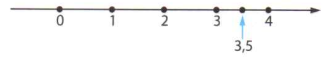
\includegraphics[width=1\linewidth]{6FMA07_imagens/imagem01} \\
		Na fração $\frac{a}{b}, a$ é o numerador e $b$ é o denominador. \\
		Para localizar uma fração $\frac{a}{b}$ na reta, dividimos o intervalo de 0 a 1 em $b$ partes iguais e, a partir do zero, contamos $a$ dessas partes. Por exemplo: na figura abaixo, localizamos a fração $\frac{3}{4}$. \\
		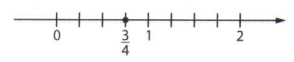
\includegraphics[width=1\linewidth]{6FMA07_imagens/imagem02} \\
		Quando o denominador de uma fração for maior que 10, ao lê-la ou escrevê-la com palavras, dizemos (ou escrevemos) o número acrescentado da palavra \textbf{avo} (ou \textbf{avos}). Por exemplo, $\frac{4}{13}$ lê-se "quatro treze avos".
		\noindent\textsubscript{-----------------------------------------------------------------------}
		\begin{enumerate} 
			\item Escreva a fração que representa a parte destacada do quadrado desenhado a seguir. \\
			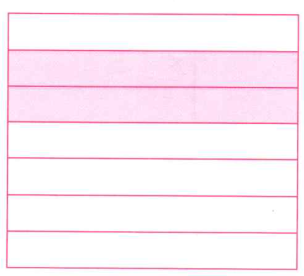
\includegraphics[width=1\linewidth]{6FMA07_imagens/imagem03} \\
			\item Carlinhos repartiu seu chocolate em 5 pedaços iguais e comeu 2 desses pedaços. Quanto ele comeu? \\\\\\\\\\\\\\\\\\\\
			\item Observe os dois exemplos abaixo, que mostram como são lidas algumas frações:
			\begin{itemize}
				\item $\frac{1}{2} \longrightarrow$	um meio (ou "meio");
				\item $\frac{1}{3} \longrightarrow$ um terço.
			\end{itemize}
			Escreva como se lê cada fração abaixo:
			\begin{enumerate}[a)]
				\item $\frac{1}{5} \longrightarrow$
				\item $\frac{1}{9} \longrightarrow$
				\item $\frac{1}{7} \longrightarrow$
				\item $\frac{1}{6} \longrightarrow$
				\item $\frac{1}{4} \longrightarrow$
				\item $\frac{1}{8} \longrightarrow$
				\item $\frac{1}{10} \longrightarrow$
			\end{enumerate}
			\item Localize $\frac{1}{3}$ na reta abaixo. \\
			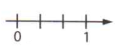
\includegraphics[width=0.5\linewidth]{6FMA07_imagens/imagem04} \\
			\item Localize a fração $\frac{3}{4}$ na reta abaixo. \\
			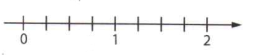
\includegraphics[width=1.1\linewidth]{6FMA07_imagens/imagem05} \\
			\item Escreva a fração $\frac{3}{8}$ como soma de frações de numerador 1.
			%24 a 29
			\item Escreva a fração que representa a parte destacada da figura abaixo. \\
			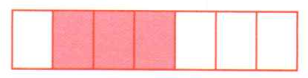
\includegraphics[width=1.1\linewidth]{6FMA07_imagens/imagem06} \\
			\item Localize $\frac{1}{6}$ na reta abaixo. \\
			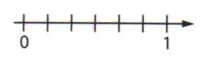
\includegraphics[width=1\linewidth]{6FMA07_imagens/imagem07} \\\\
			\item Escreva como se leem as frações abaixo.
			\begin{enumerate}[a)]
				\item $\frac{3}{4} \longrightarrow$
				\item $\frac{7}{8} \longrightarrow$
				\item $\frac{2}{5} \longrightarrow$
				\item $\frac{5}{6} \longrightarrow$
			\end{enumerate}
			\item Escreva $\frac{4}{7}$ como soma de frações de numerador 1. \\\\\\\\\\
			\item Nas retas abaixo, localize: 
			\begin{enumerate}[a)]
				\item $\frac{2}{7}$ \\
				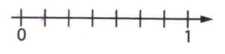
\includegraphics[width=1\linewidth]{6FMA07_imagens/imagem08} \\\\\\
				\item $\frac{5}{9}$ \\
				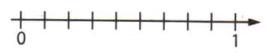
\includegraphics[width=1\linewidth]{6FMA07_imagens/imagem09} 
				\item $\frac{3}{8}$ \\
				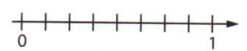
\includegraphics[width=1\linewidth]{6FMA07_imagens/imagem10} \\\\\\
			\end{enumerate}
			\item Abaixo temos duas pilhas de caixotes iguais. A pilha da direita representa que fração da pilha da esquerda?
			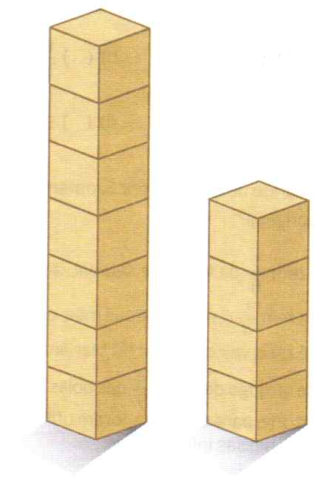
\includegraphics[width=1\linewidth]{6FMA07_imagens/imagem11} \\\\\\
		\end{enumerate}
		$~$ \\ $~$ \\ $~$ \\ $~$ \\ $~$ \\ $~$ \\ $~$ \\ $~$ \\ $~$ \\ $~$ \\ $~$ \\ $~$ \\ $~$ \\ $~$ \\ $~$ \\ $~$ \\ $~$ \\ $~$ \\ $~$ \\ $~$ \\ $~$ \\ $~$ \\ $~$ \\ $~$ \\ $~$ \\ $~$ \\ $~$ \\ $~$ \\ $~$ \\ $~$ \\ $~$ \\ $~$ \\ $~$ \\ $~$ \\ $~$ \\ $~$ \\ $~$ \\ $~$ \\ $~$ \\ $~$ \\ $~$ \\ $~$ \\ $~$ \\ $~$ \\ $~$ \\ $~$ \\ $~$ \\ $~$ \\ $~$ \\ $~$ \\ 
	\end{multicols}
\end{document}